\section{Compute Accounting and Instrumentation Semantics}
\label{sec:compute}

Table~\ref{tab:resource} and Figure~\ref{fig:tradeoff} evaluate the accounting semantics of equal
Class~A nominal budget $B{=}6$. Following Section~\ref{sec:problem}, we separate (i)~nominal
logical actions, (ii)~successful provider completions on the reported path, (iii)~internal HTTP
retries, (iv)~generated-token fields, (v)~observed latency, and (vi)~estimated dollar cost. The
columns are intentionally not collapsed: an instrumentation defect can change resource conclusions
while leaving extracted answers and accuracy unchanged.

\begin{table}[tbp]
\centering
\footnotesize
\setlength{\tabcolsep}{4pt}
\caption{Mean realized resources per evaluated Class~A policy across $15$ cells (nominal $B{=}6$).
Class~B pool cost inherits up to four Class~A pipelines (Table~\ref{tab:main-matrix}). USD uses a
2026-07-16 pricing snapshot. Frontier token/cost reconstruction status is documented in the table
note.}
\label{tab:resource}
% Auto-generated from validated corrected resource-accounting summaries.
% Class A generators only. Class B (FTA, Pooled-4) add 0 marginal calls; pool cost = sum of generators.
% Frontier calls column corrected from reconstructed successful-call counts.
% (accounting-instrumentation fix + historical reconstruction from existing raw records; no
% accuracy/answer/statistical result changed). Tokens/cost remain a documented Frontier lower
% bound; see footnote in Section~\ref{sec:compute}.
\begin{tabular}{@{}lrrrr@{}}
\toprule
Class~A method & Tokens/ex.$^\dagger$ & Latency (s) & Calls (nom.=6) & Cost/ex.$^\dagger$ (\$) \\
\midrule
Frontier & 1287.0$^\dagger$ & 16.87 & 5.38 & 0.00258$^\dagger$ \\
L1-style adapter & 728.7 & 5.48 & 1.61 & 0.00133 \\
S1-inspired adapter & 1236.0 & 8.80 & 2.85 & 0.00234 \\
TALE-EP-style adapter & 727.3 & 5.33 & 1.66 & 0.00129 \\
\bottomrule
\end{tabular}

{\scriptsize $^\dagger$Frontier tokens/cost are a documented lower bound (challenger-expansion-phase
tokens are not recoverable from historical records without fabrication); calls, latency, and all
adapter figures are complete. See Section~\ref{sec:compute}.}

\end{table}

Table~\ref{tab:resource} reports unweighted means of per-cell means. Class~B end-to-end cost
inherits up to four Class~A pipelines.

\paragraph{Instrumentation audit and successful-call reconstruction}
A harness gap reset/read usage on Frontier's outer generator only, omitting the challenger-expansion
generator. On preserved validated Frontier records, successful calls reconstruct as outer successful
calls plus \texttt{frontier\_candidate\_maturity} (maturity $=$ challenger expansions $+$ verifier
calls). Mean successful calls rise from $2.78$ to $5.38$ of nominal $B{=}6$ (example-weighted
$5.44$). Ratios versus the evaluated adapters: Frontier/L1-style~$2.13\times$--$5.18\times$,
Frontier/TALE-style~$2.03\times$--$5.51\times$, Frontier/S1-inspired~$1.43\times$--$2.50\times$
(Frontier higher in every cell). Challenger-phase tokens were never persisted, so Frontier token and
USD ratios are lower bounds ($1.22\times$--$2.56\times$ vs.\ L1-style; $1.13\times$--$2.93\times$
vs.\ TALE-style; mixed vs.\ S1-inspired); paid retries are likewise incomplete. Accuracy and
McNemar/Holm tests are unchanged. The audit supports the claim that matched $B{=}6$ did not produce
matched realized call allocations (\ref{app:compute-detail}).

\begin{figure}[tbp]
\centering
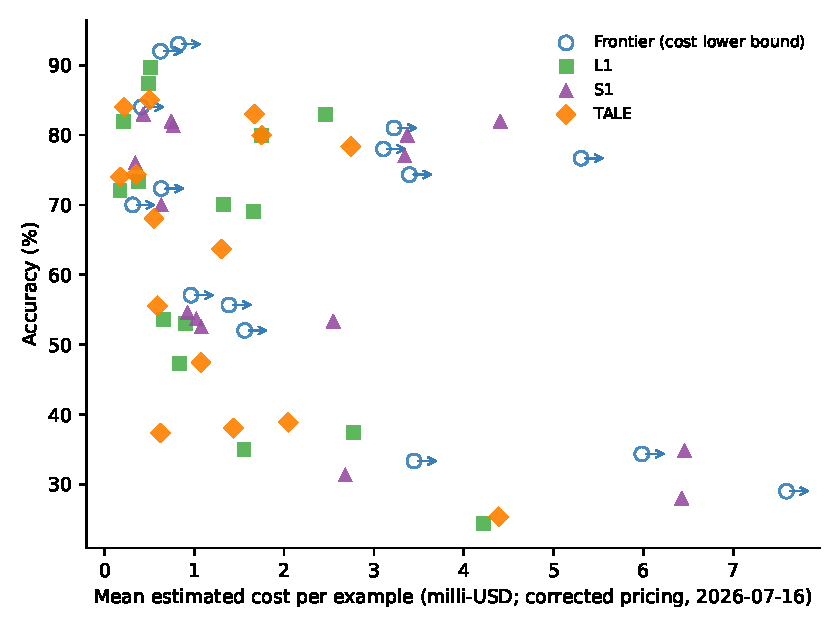
\includegraphics[width=0.80\linewidth]{figures/figure4_accuracy_vs_cost_tradeoff}
\caption{Class~A accuracy vs.\ mean estimated cost per example (milli-USD) for the evaluated
adapters under this protocol. Points occupy a tradeoff region. Open Frontier markers with rightward
arrows mark incomplete challenger-phase token persistence.}
\label{fig:tradeoff}
\end{figure}

Figure~\ref{fig:tradeoff} visualizes that tradeoff. The single-cell Azure$\times$GSM8K SC comparison
(Section~\ref{sec:sc-entitlement-control}) remains call/sample-budget-matched only.
